\chapter{Grafisk teori}

For at kunne udvikle en brugbar grafisk brugergrænseflade er det nødvendigt at forstå teorier bag dette. 
Derfor vil dette blive beskrevet i følgende kapitel. 

\section{Grafisk brugergrænseflade} \label{chap:GUI}

Centralt for systemets design, er at brugerne kan navigere rundt i det. 
Da Sejlklubben Sundets medlemmer kan bestå af en mangfoldig gruppe af mennesker, er det svært at indskrænke brugerne i en enkelt gruppe, dermed formodes det at IT-evnerne kan være meget forskellige.


\subsection{Designet} \label{sec:Designet}

Programmets brugergrænseflade vil blive designet ud fra principperne i følge Kang og Kims fortolkning. \citep{gui1} 

\begin{itemize}
	\item Minimalisme
	\item Konsistent design (Fra engelsk: Consistency)
\end{itemize}

Minimalisme betyder, at der skal være så få forstyrrelser på skærmbilledet som muligt. 
Det skal være enkelt og simpelt at navigere rundt og finde de funktioner i programmet, man skal bruge. Knapper skal gerne være holdt til et minimum og mindre brugte funktioner gemmes derfor væk i menuer eller andre vinduer.
En sådan struktur skal dog ikke have et hierarki, der er dybere end tre niveauer for ikke at gemme funktioner for brugeren.
Unødvendige ikoner og lange sætninger er således også kun til forvirring for brugeren og skal gerne undgås.
Tekst, der forekommer på brugergrænsefladen, skal også gerne være konsistente, dette gælder hele brugergrænsefladen: Farver, funktionstyper der tilføjer eller fjerner elementer, samt teksttype og størrelse for at undgå forvirring for brugeren.
Således skal den samme navigationsstruktur også være tilbagevendende igennem brugergrænsefladen.

Disse forskellige principper eller retningslinjer, er forsøgt implementeret i systemet.


\subsection{Implementation}\label{sec:Implementation}

Menustrukturen består af tabs, som er store og lette at se.
De forskellige funktioner i programmet er delt op i deres tilhørende tabs, og man kan altid gå ind i en ny tab uanset hvor, man befinder sig i programmet. 
Dette betyder, at programmet ikke har et dybt vindueshierarki.
Brugergrænsefladen vil blive testet i brugertesten, beskrevet i \myref{test_af_program}.

\section{Valg af grafikframework} 
Dette afsnit omhandler udvalgte valgmuligheder for udviklingen af brugergrænsefladen, samt valget af det endelige framework.

\subsection{Windows Presentation Foundation}
\ac{WPF} er en grafisk framework på Windowsbaserede applikationer. 
WPF gør brug af moderne teknologier til at generere grafik, bl.a. vektorbaseret og hardware accelereret rendering.
Visual Studio har en indbygget designer til WPF, hvilket simplificerer udviklingsprocessen. 
Grafikken kan enten defineres i \ac{XAML}--formatet eller ved C\#--kode. 
Fordele ved \ac{XAML}--formatet er en adskillelse af logik og grafik. 
Hvis grafikken kun er defineret som C\#--kode kan det være svært at bevare overblikket, når kompleksiteten øges.
Selve C\#-koden, den såkaldte Code--Behind, ligger i en separat fil, med samme navn som XAML-filen. 
Hvis der f.eks. er skabt en Button, en almindelig knap, i XAML-filen, så vil det kode, som Button'en skal udføre, blive placeret i Code-Behind-filen, som består af C\#--kode, så grafikken og koden bliver hver for sig, hvilket kan give et bedre overblik \citep{wpf}. 

\subsection{Windows Forms}
Windows Forms (WinForms) er, som \ac{WPF}, et grafisk framework til udvikling på Windows platformen, som en overbygning til Windows API.
WinForms er forgængeren til WPF, hvilket betyder at WPF har nogle nye features, som WinForms ikke har.
WinForms har ikke et tilknyttet markup sprog, så selve grafikken skal skrives sammen med selve koden. 
\citep{winforms2}

\subsection{Website}
En anden mulighed, som blev diskuteret, var at bruge en hjemmeside, som ville have den fordel, at den kan køre på stort set alle enheder, som har adgang til internettet via en browser. 
En hjemmeside, som gør brug af C\#, vil kunne laves på en måde, som minder om den ved WPF og XAML; med HTML (HyperText Markup Language), JS (JavaScript) og CSS (Cascading Style Sheets) som front end og C\#--kode som back end. 

\subsection{Afgrænsning}
En hjemmeside blev fravalgt, da det blev vurderet at WPF var nemmere at oprette end en hjemmeside.
Samtidig er fokus rettet mod objektorienterede principper fremfor udvikling af brugergrænseflade.

WinForms blev fravalgt, da det er ved at være forældet.
Microsoft har informeret om, at der ikke længere tilføjes nye funktioner til WinForms, men at der udelukkende bliver lavet rettelser af fejl.\citep{winforms}

I dette projekt bruges \ac{WPF} til at skabe den grafiske brugergrænseflade. 
Valget faldt på \ac{WPF}, da dets integration i Visual Studio simplificerer det skabelsen af en grafisk brugergrænseflade.


\begin{wrapfigure}[22]{r}{0.5\textwidth}
    \label{img:wpfdemo}
    \vspace{-30pt}
    \begin{center}
        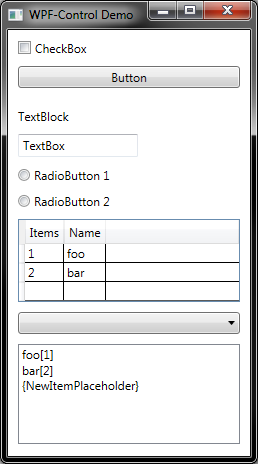
\includegraphics[width=0.48\textwidth]{UI/WPF-Demo.png}
    \end{center}
    \vspace{-15pt}
    \caption{Demonstration af WPFs Controls}
    \vspace{-15pt}
\end{wrapfigure}

\subsection{Ofte anvendte WPF-controls}
I projektet anvendes bestemte WPF controls til at bygge brugergrænsefladen. 
De hyppigst anvendte vil her blive beskrevet. 
På figur \ref{img:wpfdemo} vises de beskrevne elementer.


\subsubsection*{ComboBox}
I WPF er en ComboBox det element, som andre steder omtales som en dropdown menu. 
Dens indhold kan indstilles enten i XAML-koden eller i Code-Behind koden.
Hvis dette indhold skal være dynamisk, kan man anvende Code-Behind, eksempelvis hvis man kun vil have de medlemmer af en liste, som opfylder et givent prædikat.


\subsubsection*{Button}
En Button er en knap, som kalder en metode i Code-Behind, når den trykkes på.

\subsubsection*{DataGrid}
Et DataGrid er et grafisk element, som kan vise data på tabelform.
Ofte vil det vise en liste af objekter.
Dets layout er opdelt i rækker og kolonner, hvor hver kolonne indeholder en bestemt type data, og kan sorteres ved at klikke på de forskellige headers.
Det er også muligt at konstruere en søgefunktion, altså kan et DataGrid blive filtreret.

\subsubsection*{CheckBox}
En CheckBox er en kvadratisk boks, som enten er ``Checked'' eller ``UnChecked''.
I code--behind kan stadiet af en CheckBox aflæses.

\subsubsection*{RadioButton}
En RadioButton er en cirkelformet CheckBox.
Dog vil RadioButtons ofte optræde i serie, altså to eller flere sammen, da valget af den ene ekskluderer valget af de andre. 
Et oplagt brug af dem er til ja, nej (og måske) situationer, hvor kun en af dem skal vælges.

\subsubsection*{TextBlock}
En TextBlock bruges til visning af tekst, som ikke kan redigeres.
Det vil typisk være en forklarende tekst op ad et andet grafisk element.
Det er også muligt at ændre en TextBlock via Code-Behind, hvis man vil føre en dialog med brugeren, eksempelvis til fejlbeskeder.

\subsubsection*{TextBox}
En TextBox er et tekstfelt, hvori brugeren kan indtaste tekst. 
Dette kan dermed ses som et inputfelt. 
Det er også muligt at sætte sådan et felt til at være skrivebeskyttet, så brugeren ikke kan redigere det, imens programmet stadig kan ændre feltets indhold.

\subsubsection*{ListBox}
En ListBox er en liste, hvori en bruger kan vælge en eller flere elementer.
ListBoxen er i stand til at indeholde samlinger af data på enhver form, oftest vil det være en streng, men et billede er også en mulighed.
Den vil i nogle tilfælde have samme brugsscenarie som en ComboBox eller et DataGrid. 
Forskellen fra en ComboBox er, at der kan være flere synlige elementer i en ListBox på samme tid, samt der ikke er nogen dropdown menu.

\subsubsection*{UserControls}
Det er muligt at konstruere sine egne grænsefladeelementer fra et eller flere af WPFs indbyggede eller 3. parts Controls.
Dette kaldes en UserControl, som indeholder både en grafisk del og en Code-Behind del.
Det brugerskabte element kan derefter genbruges flere steder i programmet.
Dette er et eksempel på genanvendelse, hvilket kan bidrage til højere programkvalitet og større konsistens gennem programmet. 

\subsection*{Vinduer}
Et vindue er det som indkapsles af kanter og knapperne minimer, maksimer, luk findes på Windows i øverst i højre hjørne.
I vinduer indsættes alle de ovenstående elementer, for at skabe og vise den grafiske brugergrænseflade.
